% !TEX root = ../report.tex

\chapter{Архітектура та методологія побудови системи керованої колоризації}
    \label{chap:implementation}
        У цьому розділі представлено опис спроєктованої системи інтерактивної колоризації зображень, що базується на інтеграції SSM та U-Net архітектур.
        Розглядається методологія підготовки даних, принципи формування та кодування користувацьких підказок, а також загальний конвеєр обробки інформації. 
        
        Окрему увагу приділено компонентній деталізації розробленої гібридної моделі, математичному обґрунтуванню механізмів двонаправленого сканування та оптимізації функцій втрат для забезпечення стабільного навчання.

    \section{Загальна концепція та конвеєр обробки даних системи}
        Розроблена система інтерактивної колоризації функціонує в межах конвеєра обробки на основі підказок,
        який поєднує автоматичне вилучення семантичних ознак монохромного зображення із просторовим керуванням через визначені користувачем точкові орієнтири.
        
        На відміну від повністю автоматичних методів, які розв'язують задачу <<один до багатьох>> виключно на основі апріорних знань нейромережі,
        запропонований підхід дозволяє задавати цільові кольори для конкретних семантичних областей зображення,
        трансформуючи задачу у стохастичну генерацію з граничними умовами.

        Математично вхідний потік даних формується шляхом злиття інформації з двох різних модальностей:
        \begin{enumerate}
            \item \textbf{Канал яскравості:} Одноканальне чорно-біле зображення $I_L \in \mathbb{R}^{1 \times H \times W}$, вилучене як компонент $L$ колірного простору $\mathrm{CIELAB}$ та нормалізоване до $[-1, 1]$.
            \item \textbf{Тензор підказок (Hints):} Триканальний просторовий масив $I_{\mathrm{hints}} \in \mathbb{R}^{3 \times H \times W}$, який кодує хроматичну інформацію у точках взаємодії користувача з інтерфейсом.
        \end{enumerate}

        Для того, щоб нейромережа могла чітко диференціювати точки, де користувач свідомо задав колір, від порожнього простору, тензор підказок $I_{\mathrm{hints}}$ розділяється на:
        \begin{itemize}[label=$\bullet$]
            \item Канали кольоровості $a$ та $b$, розмірності $2 \times H \times W$, нормалізовані у $[-1, 1]$, які містять цільові хроматичні значення у координатах заданих точок, а у решті пікселів заповнені нулями.
            \item Маску інтенсивності підказок $M \in [0, 1]^{1 \times H \times W}$, де значення більше певного шуму, близького до $0$, наприклад $0.05$, є користувацькою підказкою, а менше певного шуму вказує на відсутність в цьому місці підказки.
                Без використання цього каналу модель сприймала б нулі у порожніх зонах як вимогу розфарбувати всю картинку у нейтральний сіро-зелений колір.
        \end{itemize}

        Перед подачею в енкодер канали об'єднуються вздовж виміру каналів за допомогою операції конкатенації,
        утворюючи уніфікований чотириканальний тензор $X_{\mathrm{in}} = \mathrm{Concat}(I_L, I_{\mathrm{hints}}) \in \mathbb{R}^{4 \times H \times W}$.

        \subsection{Стратегія симуляції підказок користувача під час навчання}
            Оскільки під час реального використання кількість, розмір та розташування точок є випадковими,
            процес навчання моделі вимагає динамічної симуляції дій користувача на кожній ітерації.
            Навчання на фіксованих шаблонах призвело б до перенавчання моделі та ігнорування підказок на інференсі.

            Конвеєр підготовки даних під час тренування реалізує таку стохастичну процедуру для кожного батчу:
            \begin{enumerate}
                \item З оригінального кольорового зображення вилучаються істинні канали кольоровості $Y \in \mathbb{R}^{2 \times H \times W}$.
                \item Випадковим чином визначається цільова кількість підказок $K$ з дискретного геометричного розподілу $K \sim \mathrm{Geom}(p=0.2)$,
                    в якому математичне сподівання становить $\mathbb{E}[K] = \frac{1 - p}{p}$, тобто в середньому генерується $4$ підказки. Ймовірність появи конкретної кількості підказок $k$ обчислюється як $P(K=k) = p \cdot (1-p)^k$. Зокрема, ймовірність генерації зображення взагалі без підказок, $K=0$, становить $20\%$, що змушує модель також вчитися безумовній автоматичній колоризації.
                \item Для імітації людської уваги координати генеруються алгоритмом виділення візуальної значимості. Додатково застосовується евристика мінімальної просторової відстані, яка відкидає нові координати, якщо вони знаходяться занадто близько до вже існуючих, уникаючи неприродного скупчення кліків.
                \item Формується маска інтенсивності $M$: у вибраних координатах розміщуються двовимірні радіальні гаусові ядра випадкового радіуса та випадкової амплітуди інтенсивності (від $0.2$ до $1.0$). Це імітує різні розміри пензля користувача та ступінь <<впевненості>> підказки.
                    Якщо гаусові плями перекриваються, маска оновлюється за принципом максимуму $M_{new} = \max(M_{old}, G_{patch})$.
                \item Формуються канали підказок $a$ та $b$ шляхом поелементного множення істинних значень $Y$ на згенеровану маску $M$.
            \end{enumerate}

        \subsection{Автоматизована симуляція підказок на етапі валідації}
            Для об'єктивної оцінки якості моделі під час валідації та тестування, алгоритм перемикається з випадкової генерації у детермінований <<експертний>> режим. Алгоритм автоматично знаходить найбільш інформативні зони для колоризації, діючи за такою логікою:
            \begin{enumerate}
                \item Обчислюється матриця спектральної магнітуди, насиченості кольору, для всього зображення як сума квадратів значень каналів $a$ та $b$.
                \item Визначаються координати пікселя з максимальною магнітудою, і в цій точці розміщується гаусова підказка фіксованого розміру.
                \item Щоб запобігти вибору точок в одному й тому самому об'єкті, застосовується механізм просторового пригнічення: значення магнітуди в заданому радіусі навколо обраної точки примусово встановлюються у від'ємні значення ($-1.0$).
                \item Процес ітеративно повторюється для заданої кількості підказок, наприклад, $K=3$.
            \end{enumerate}
            Такий конвеєр валідації гарантує, що модель отримує підказки саме в найскладніших, найбільш яскравих ділянках зображення, що дозволяє коректно оцінити її здатність до поширення кольору на великі просторові відстані.

    \section{Компонентна деталізація та алгоритми навчання гібридної моделі}
        % Що сюди пишемо:
        % 1. Анатомія MambaWrapper та DoubleConv (можна вставити твій код або його табличний опис).
        % 2. Математика bidirectional сканування (обґрунтування твого torch.flip).
        % 3. Механізм MambaShared (як реалізовано layer sharing).
        % 4. Формули лос-функцій (комбінація цільової похибки та контурів).

% У цьому розділі описується практична реалізація розробленої системи інтерактивної колоризації на основі запропонованого методу. На основі аналізу, проведеного у попередніх розділах, за базову архітектуру було обрано гібридну нейронну мережу, що поєднує просторову точність згорткових мереж (U-Net) з лінійною ефективністю та глобальним рецептивним полем моделей простору станів (Mamba-SSM).

% Загальна архітектура розробленої мережі представлена на рис.~\ref{fig:arch_general}. Детально розглядається архітектурна формалізація процесу, проєктування базових блоків мережі, алгоритм інтеграції користувацьких підказок у латентний простір, а також механізм двонаправленого сканування (Bidirectional Scan) для усунення просторової асиметрії. 

% \begin{figure}[ht]
%     \centering
%     \resizebox{\textwidth}{!}{%
%     \begin{tikzpicture}[
%         scale=0.8, transform shape,
%         box/.style={draw, thick, rounded corners=3pt, align=center, minimum width=2.5cm, minimum height=0.9cm, font=\small},
%         enc/.style={box, fill=blue!10, draw=blue!60!black},
%         dec/.style={box, fill=cyan!10, draw=cyan!60!black},
%         skip/.style={->, thick, dashed, color=gray!80!black, >=stealth},
%         arr/.style={->, thick, color=black, >=stealth}
%     ]
%         % --- Input ---
%         \node[box, fill=gray!15, draw=gray!60!black, minimum width=2cm] (in) at (-5, 0) {\textbf{Вхід}\\$L$ + $ab_{hint}$ + маска\\(4 канали)};

%         % --- ENCODER ---
%         \node[enc] (enc1) at (-1, 0) {\textbf{Enc 1} (DoubleConv)\\$64$ каналів, $H \times W$};
%         \node[enc] (enc2) at (-1, -1.5) {\textbf{Enc 2} (DoubleConv)\\$128$ каналів, $\frac{H}{2} \times \frac{W}{2}$};
%         \node[enc] (enc3) at (-1, -3) {\textbf{Enc 3} (DoubleConv)\\$256$ каналів, $\frac{H}{4} \times \frac{W}{4}$};

%         % --- BI-MAMBA ---
%         \node[box, fill=green!10, draw=green!60!black, minimum width=6cm, minimum height=2.2cm] (mamba) at (2.5, -5) {};
%         \node[above, font=\footnotesize\bfseries, color=black] at (mamba.north) {Bi-Directional Mamba};
        
%         \node[box, fill=white, draw=green!80!black, minimum width=2.2cm, minimum height=0.6cm, font=\footnotesize] (mfwd) at (1, -4.5) {Mamba Fwd};
%         \node[box, fill=white, draw=green!80!black, minimum width=2.2cm, minimum height=0.6cm, font=\footnotesize] (mrev) at (2.85, -5.5) {Mamba Rev};
%         \node[circle, draw=black, thick, fill=white, inner sep=1pt, font=\small] (plus) at (4.6, -4.5) {$+$};
%         \node[above, font=\scriptsize, text=black] at (plus.north) {Усереднення};

%         \draw[arr, color=black] (mfwd) -- (plus);
%         \draw[arr, color=black] (mrev) -- (4.6, -5.5) -- (plus);

%         % --- DECODER ---
%         \node[dec] (dec3) at (6, -3) {\textbf{Dec 3} (DoubleConv)\\$128$ каналів, $\frac{H}{4} \times \frac{W}{4}$};
%         \node[dec] (dec2) at (6, -1.5) {\textbf{Dec 2} (DoubleConv)\\$64$ каналів, $\frac{H}{2} \times \frac{W}{2}$};
%         \node[dec] (dec1) at (6, 0) {\textbf{Dec 1} (DoubleConv)\\$64$ каналів, $H \times W$};

%         % --- OUTPUT ---
%         \node[box, fill=orange!15, draw=orange!60!black, minimum width=2cm] (out) at (10, 0) {\textbf{Вихід}\\Канали $a, b$\\$[-1, 1]$};

%         % --- Arrows ---
%         \draw[arr] (in) -- (enc1);

%         \draw[arr] (enc1) -- node[right, font=\scriptsize] {Pool $\downarrow 2$} (enc2);
%         \draw[arr] (enc2) -- node[right, font=\scriptsize] {Pool $\downarrow 2$} (enc3);

%         \draw[arr] (enc3) -- node[left, font=\scriptsize, align=right] {Pool $\downarrow 2$\\Flatten\\$\to (B, L, D)$} (-1, -5) -- (mamba.west);
        
%         \draw[arr, color=black] (mamba.west) -- (mfwd.west);
%         \draw[arr, color=black] (mfwd.south) -- node[left, font=\scriptsize] {Flip} (1, -5.5) -- (mrev.west);
%         \draw[arr, color=black] (plus.east) -- (mamba.east);

%         \draw[arr] (mamba.east) -- (6, -5) -- node[right, font=\scriptsize, align=left] {Reshape\\Up $\uparrow 2$} (dec3.south);

%         \draw[arr] (dec3) -- node[right, font=\scriptsize] {Up $\uparrow 2$} (dec2);
%         \draw[arr] (dec2) -- node[right, font=\scriptsize] {Up $\uparrow 2$} (dec1);

%         \draw[arr] (dec1) -- node[above, font=\scriptsize] {1x1 Conv} node[below, font=\scriptsize] {Tanh} (out);

%         \draw[skip] (enc1) -- node[above, font=\scriptsize, text=gray!80!black] {Concat} (dec1);
%         \draw[skip] (enc2) -- node[above, font=\scriptsize, text=gray!80!black] {Concat} (dec2);
%         \draw[skip] (enc3) -- node[above, font=\scriptsize, text=gray!80!black] {Concat} (dec3);

%     \end{tikzpicture}%
%     }
%     \caption{Архітектура гібридної нейронної мережі Bidirectional Shared Mamba}
%     \label{fig:arch_general}
% \end{figure}

% \section{Формулювання задачі інтерактивної колоризації}

% Класична задача безумовної колоризації має фундаментальну проблему — надмірну невизначеність. Одному чорно-білому зображенню (канал яскравості $L$ у просторі CIELAB) може відповідати нескінченна кількість правдоподібних кольорових варіацій (канали $a$ та $b$). Використання лише базових функцій втрат, таких як середньоквадратична похибка, змушує модель усереднювати всі можливі кольори, що призводить до генерації тьмяних зображень (відомий як ефект «сепії»).

% Для вирішення цієї проблеми та забезпечення багатоваріантності результатів розроблена система формулюється як задача умовної генерації (Conditional Generation). Модель навчається апроксимувати функцію відображення:
% \begin{equation*}
%     F: (L, H_{ab}, M) \rightarrow (\hat{a}, \hat{b}),
% \end{equation*}
% де $L$ — вхідний канал яскравості розмірності $H \times W \times 1$; $H_{ab}$ — тензор користувацьких підказок розмірності $H \times W \times 2$; $M$ — бінарна маска розмірності $H \times W \times 1$, яка вказує на просторове розташування дійсних підказок; $(\hat{a}, \hat{b})$ — прогнозовані хроматичні канали.

% Для того, щоб уникнути появи жорстких артефактів у місцях кліків користувача, підказки розмиваються за допомогою двовимірного ядра Гаусса, утворюючи м'які плями розподілу кольору, які нейромережа здатна плавно поширювати до найближчих семантичних меж об'єктів. Загальний вхідний тензор має 4 канали і подається на вхід енкодера.

% \section{Архітектура запропонованої моделі Bi-Mamba}

% Розроблена модель базується на ієрархічній структурі типу U-Net, де класичний центральний вузол (Bottleneck) замінено на інноваційний блок простору станів.

% \subsection{Проєктування енкодера та декодера (DoubleConv)}
% Для вилучення просторових ознак та поступового зниження роздільної здатності використовується згортковий енкодер, що складається з трьох рівнів. Кожен рівень побудований на базі абстракції \textit{DoubleConv}, структурну схему якої зображено на рис.~\ref{fig:doubleconv}.

% \begin{figure}[ht]
%     \centering
%     \resizebox{0.9\textwidth}{!}{%
%     \begin{tikzpicture}[
%         scale=0.9, transform shape,
%         layer/.style={draw, thick, rounded corners=3pt, align=center, font=\small, text=black, minimum width=2.6cm, minimum height=1cm},
%         conv/.style={layer, fill=blue!10, draw=blue!40!black},
%         bn/.style={layer, fill=orange!10, draw=orange!40!black},
%         relu/.style={layer, fill=green!10, draw=green!40!black},
%         io/.style={layer, fill=gray!10, draw=gray!40!black},
%         arr/.style={->, thick, color=black, >=stealth},
%         group_box/.style={draw, dashed, thick, color=gray, rounded corners=5pt}
%     ]
%         % --- ВХІД ---
%         \node[io] (in) at (-1.5, 0) {\textbf{Вхід $x$}\\$C_{in} \times H \times W$};
%         % --- РЯДОК 1 ---
%         \node[conv] (c1) at (2.5, 0) {\textbf{Conv2d} ($3\times3$)\\$C_{in} \to C_{out}$};
%         \node[bn] (b1) at (6.2, 0) {\textbf{BatchNorm2d}\\$C_{out}$};
%         \node[relu] (r1) at (9.9, 0) {\textbf{ReLU}};
%         % --- РЯДОК 2 ---
%         \node[conv] (c2) at (2.5, -2.5) {\textbf{Conv2d} ($3\times3$)\\$C_{out} \to C_{out}$};
%         \node[bn] (b2) at (6.2, -2.5) {\textbf{BatchNorm2d}\\$C_{out}$};
%         \node[relu] (r2) at (9.9, -2.5) {\textbf{ReLU}};
%         % --- ВИХІД ---
%         \node[io] (out) at (13.8, -2.5) {\textbf{Вихід $y$}\\$C_{out} \times H \times W$};
        
%         % --- СТРІЛКИ ДАНИХ ---
%         \draw[arr] (in) -- (c1);
%         \draw[arr] (c1) -- (b1);
%         \draw[arr] (b1) -- (r1);
%         \draw[arr, rounded corners=6pt] (r1.south) -- ++(0, -0.75) -| (c2.north);
%         \draw[arr] (c2) -- (b2);
%         \draw[arr] (b2) -- (r2);
%         \draw[arr] (r2) -- (out);
        
%         % --- РАМКА НАВКОЛО SEQUENTIAL ---
%         \draw[group_box] (0.8, 1.2) rectangle (11.6, -3.5);
%         \node[color=black, font=\bfseries] at (6.2, 1.5) {DoubleConv (nn.Sequential)};
%     \end{tikzpicture}%
%     }
%     \caption{Архітектура блоку DoubleConv для енкодера та декодера}
%     \label{fig:doubleconv}
% \end{figure}

% Блок DoubleConv включає послідовне виконання згорткового шару $3 \times 3$, шару батч-нормалізації (BatchNorm2d) та активації ReLU. Після кожного блоку DoubleConv в енкодері застосовується операція \textit{Max Pooling} ($2 \times 2$), яка зменшує просторову розмірність карт ознак у два рази. Декодер працює симетрично. Важливим елементом є використання наскрізних зв'язків (Skip Connections), які прокидають карти ознак з енкодера безпосередньо в декодер, обминаючи центральний блок для збереження дрібних деталей.

% \subsection{Інтеграція двонаправленого блоку Mamba}
% Основна інновація розробленої системи лежить у центральному вузлі архітектури. Ознаки, отримані після третього рівня енкодера розгортаються у послідовність (Flatten) і передаються до блоку простору станів. Його будову деталізовано на рис.~\ref{fig:shared_mamba}.

% \begin{figure}[ht]
%     \centering
%     \resizebox{0.9\textwidth}{!}{%
%     \begin{tikzpicture}[
%         scale=0.9, transform shape,
%         layer/.style={draw, thick, rounded corners=3pt, align=center, font=\small, text=black, minimum width=2.8cm, minimum height=1cm},
%         mamba/.style={layer, fill=green!10, draw=green!60!black},
%         norm/.style={layer, fill=orange!10, draw=orange!60!black},
%         io/.style={layer, fill=gray!10, draw=gray!60!black},
%         add/.style={circle, draw=black, thick, fill=gray!20, inner sep=2pt, font=\small, text=black},
%         arr/.style={->, thick, >=stealth, color=black},
%         braceArr/.style={draw, dashed, thick, color=gray, rounded corners=5pt},
%         shared/.style={layer, fill=green!15, draw=green!60!black, minimum width=3.2cm}
%     ]
%         % --- Рамка одного кроку ---
%         \draw[braceArr, fill=gray!5] (1.7, 1.3) rectangle (11.3, -1.8);
%         \node[font=\bfseries\small, color=black] at (6.5, 1.65) {Крок $i = 0, 1, \ldots, \texttt{layers}{-}1$};

%         % --- ВХІД ---
%         \node[io] (in) at (0, 0) {\textbf{Вхід} $x$\\$(B,\,L,\,D)$};

%         % --- КРОК i ---
%         \node[norm]   (ln)  at (3.5, 0)   {\textbf{LayerNorm$_i$}\\$D$};
%         \node[shared] (mb)  at (7.2, 0)   {\textbf{Mamba Block}\\(спільний, $\lfloor i/k \rfloor$)};
%         \node[add]    (add) at (10.5, 0)  {$+$};

%         % --- ВИХІД ---
%         \node[io] (out) at (13.5, 0) {\textbf{Вихід} $x$\\$(B,\,L,\,D)$};

%         % --- Стрілки прямого проходу ---
%         \draw[arr] (in)  -- (ln);
%         \draw[arr] (ln)  -- (mb);
%         \draw[arr] (mb)  -- (add);
%         \draw[arr] (add) -- (out);

%         % --- Residual skip ---
%         \draw[arr, rounded corners=6pt]
%             (in.south) -- ++(0, -0.5) -- node[above, font=\scriptsize, text=black] {residual} ++(10.5,0) -- (add.south);

%         % --- Пул спільних блоків ---
%         \node[font=\small\bfseries, color=black] at (7.15, -3.25) {\textit{Пул спільних блоків (\texttt{blocks} = 2)}};
%         \node[shared, minimum width=2.2cm, minimum height=0.75cm, font=\footnotesize] (b0) at (6, -2.5) {Mamba$_0$};
%         \node[shared, minimum width=2.2cm, minimum height=0.75cm, font=\footnotesize] (b1) at (8.25, -2.5) {Mamba$_1$};

%         % --- Формула індексу ---
%         \node[above, font=\scriptsize, color=green!50!black, align=left] at (mb.north) {$\text{block idx} = \min\!\left(\left\lfloor\frac{i}{\lfloor \text{Layers}/\text{Blocks} \rfloor}\right\rfloor,\, \text{Blocks}{-}1\right)$};

%         \draw[arr, dashed, color=gray, rounded corners=4pt] (b0.north) -- ++(0, 0.5) -- (mb.south);
%         \draw[arr, dashed, color=gray, rounded corners=4pt] (b1.north) -- ++(0, 0.5) -- (mb.south);

%         % --- LayerNorm пул ---
%         \node[io, minimum width=2.6cm, minimum height=0.75cm, font=\footnotesize] (lns) at (2, -2.5) {LayerNorm$_0 \ldots$ LayerNorm$_5$};
%         \node[font=\scriptsize, color=gray!80!black, align=center] at (2, -3.25) {(унікальні, \texttt{layers} = 6)};
%         \draw[arr, dashed, color=gray, rounded corners=4pt] (lns.north) -- ++(0, 0.5) -- (ln.south);

%     \end{tikzpicture}%
%     }
%     \caption{Внутрішня архітектура та механізм розділення ваг у блоці Shared Mamba}
%     \label{fig:shared_mamba}
% \end{figure}

% Базовий механізм Mamba є однонаправленим. Для подолання просторової асиметрії розроблено модуль \textbf{Bidirectional Shared Mamba}, який сканує послідовність у природному та інвертованому напрямках, використовуючи один і той самий набір параметрів із пулу блоків. Результати прямого та зворотного сканування додаються та усереднюються.

% \section{Програмне середовище та застосунок користувача}

% Програмна реалізація виконана мовою Python з використанням фреймворку PyTorch. Для демонстрації роботи системи розроблено графічний застосунок (рис.~\ref{fig:app_gui}). Застосунок дозволяє користувачеві завантажити монохромне зображення, нанести кольорові підказки за допомогою вбудованого пензля та миттєво отримати згенерований результат або серію варіацій. 

% \begin{figure}[ht]
%     \centering
%     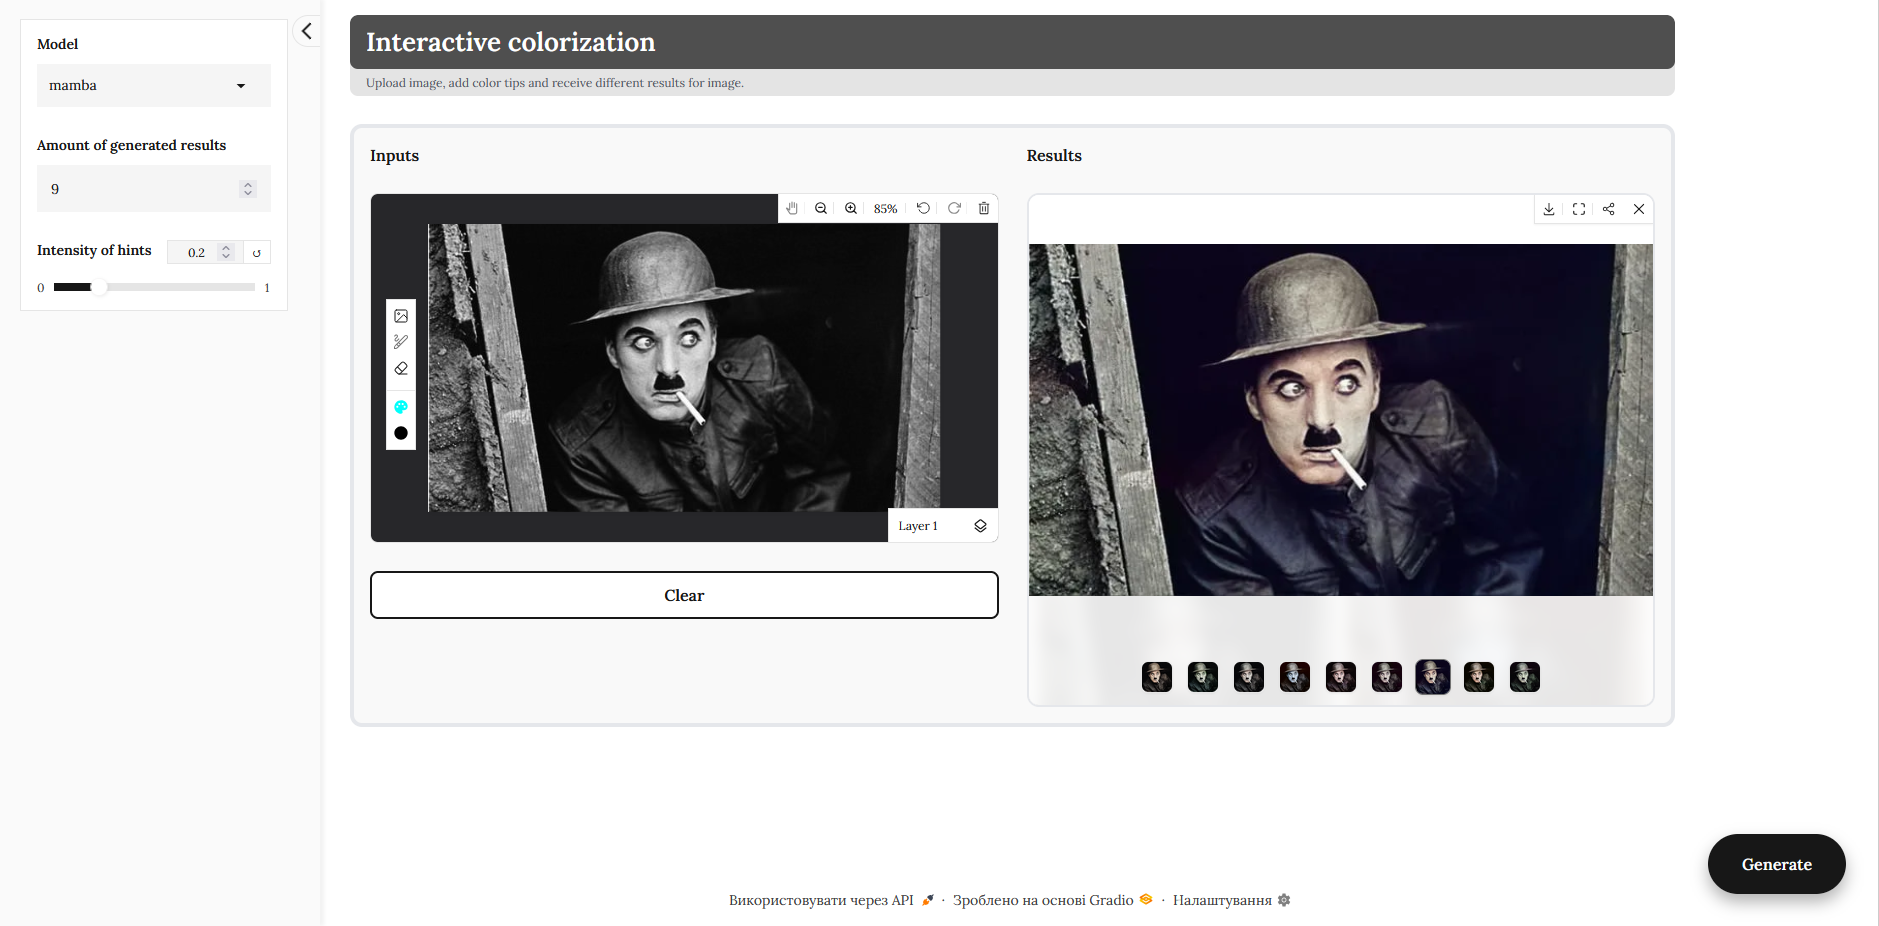
\includegraphics[width=0.85\textwidth, keepaspectratio]{images/app-image.png}
%     \caption{Інтерфейс розробленого застосунку для інтерактивної колоризації}
%     \label{fig:app_gui}
% \end{figure}

\chapconclude{\ref{chap:implementation}}
    У цьому розділі було детально описано процес інженерного проєктування та практичної реалізації системи багатоваріантної колоризації.
    Розроблено оригінальну архітектуру Bi-Mamba, яка поєднує U-Net для контролю локальних меж та двонаправлену Mamba зі спільними вагами.
    Окрім того, створено зручний графічний застосунок.